\documentclass[a4paper, oneside, 12pt]{scrbook}
\usepackage[utf8]{inputenc}
\usepackage[ngerman]{babel}
\usepackage{graphicx}
\usepackage{hyperref}
%\usepackage{minted}
\usepackage[cache=false, outputdir=build]{minted}

\pagestyle {headings}
\bibliographystyle{alphadin}



\title{Entwicklung eines Linux Gerätetreibers am Beispiel eines e-Paper Displays}
\author{Anna-Lena Marx}
\date{\today}


\begin{document}
\frontmatter
\maketitle
%abstract
% !TEX root = Projektarbeit.tex

\section*{Abstract}
%titel + autor ?
%wichtige infos
%längeren text und ergebnisse zusammenfassen
%motivation 
%fragestellung
%methoden der bearbeitung
%schlussfolgerung
\tableofcontents
\newpage

\mainmatter
%mainpart
% !TEX root = Projektarbeit.tex

\chapter{Einleitung}
Im gerade aufstrebenden Gebiet der eingebetteten Systeme spielt \textsc{Linux} nicht nur als schlankes, gut portierbares Betriebssystem eine tragende Rolle. Auch die Möglichkeit neue Hardware, beispielsweise Sensorik einfach in bestehende Systeme integrieren zu können macht Linux zu einer interessanten Plattform. 
Während in es in vielen Fällen ausreicht solche Hardware über sehr gut dokumentierte und einfach zu verwendende Schnittstellen im \texttt{Userspace} anzusprechen, gibt es doch Anwendungsfälle die Hardwaretreiber im \texttt{Kernelspace} erfordern. 

Zu letzterem zählen beispielsweise zeitkritische Treiber, die darauf angewiesen sind priorisiert und zu festen Zeitpunkten abgearbeitet zu werden, oder auch Hardwaretreiber im \textsc{Android}-Umfeld, die schon aufgrund des Designs des Systems genauer gesagt dessen Rechteverwaltung nicht im Userspace laufen dürfen. \newline

Diese Projektarbeit soll sich mit solch einem Kerneltreiber auf einem eingebettetem System beschäftigen und exemplarisch darstellen, wie ein Linux-Treiber aufgebaut ist und funktioniert. Dazu wird an einem \textsc{Beaglebone Black}, einem eingebetteten Entwicklerboard, über die \texttt{UART}-Schnittstelle ein e-Paper-Display durch ein Linux-Kernel-Modul angebunden. Das Modul soll dem Nutzer die linuxtypischen Treiberschnittstellen bereitstellen und so die Kommunikation mit der Hardware zu ermöglichen.

Der Fokus soll hierbei vor allem auf allgemeinen Prinzipien und Funktionsweisen von Linux-Treibern liegen und erklären was in diesem komplexen, wenig bekannten Bereich ablaufen muss um Hardware so selbstverständlich verwenden zu können, wie dies in heutigen Linux-Systemen der Fall ist. 
%Auf der vollständige Implementierung des Treibers liegt nicht das Hauptaugenmerk.

\chapter{Hardware}

\section{Beaglebone Black}
Zur Durchführung der Projektarbeit wird das \textsc{Beaglebone Black}, ein eingebettetes Entwicklerboard auf Basis des ARM-Prozessors AM335x von \textsc{Texas Instruments} eingesetzt. Das Beaglebone bietet mit einer Taktrate von 1GHz (Singlecore), 512MB RAM und vielen zugänglichen Hardware- und Debug-Schnittstellen, sowie einer sehr guten Dokumentation ideale Voraussetzungen für Hardwareintegration und Debugging. 

%Bild: beaglebone.org
\begin{figure}[ht]
  \centering
  \fbox{
   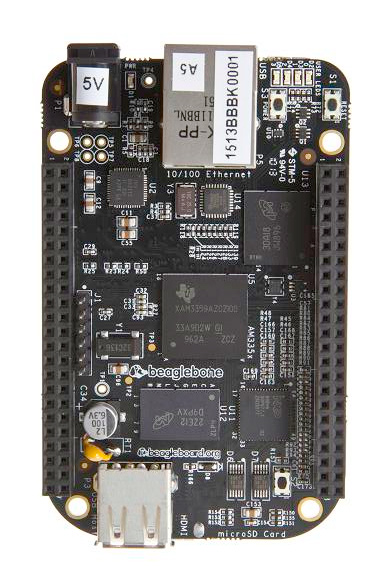
\includegraphics[angle=270, scale=0.4]{beagleboneblack_beaglebone_org}
  }
  \caption{Beaglebone Black}
  \label{pic:Beaglebone}
\end{figure}


\section{Waveshare e-Paper-Display}
Bei dem e-Paper-Display handelt es sich um ein Modell des Herstellers \textsc{Waveshare} mit einer Auflösung von 800 x 600 Pixeln und einer Größe von 4,3 inch, dass sehr einfach über die bekannte \texttt{UART}-Schnittstelle angesprochen werden kann. 
E-Paper-Displays sind vor allem dadurch interessant, dass einige Modelle wie auch das Gewählte, in der Lage sind die Anzeige auch ohne Spannungszufuhr aufrecht zu erhalten.
%TODO Was ist e-Paper, warum gewählt

%Bilder: waveshare.com
\begin{figure}
  \centering
  \fbox{
  \subfigure[e-Paper Display Front]{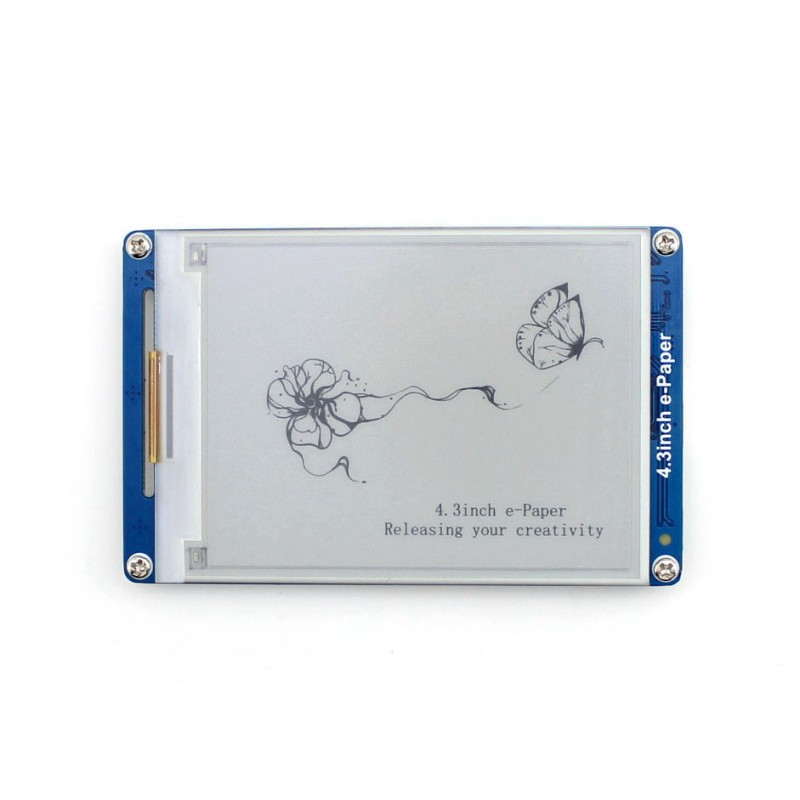
\includegraphics[scale=0.25]{43inch-e-paper-3_waveshare_com}}
  \subfigure[Rückseite]{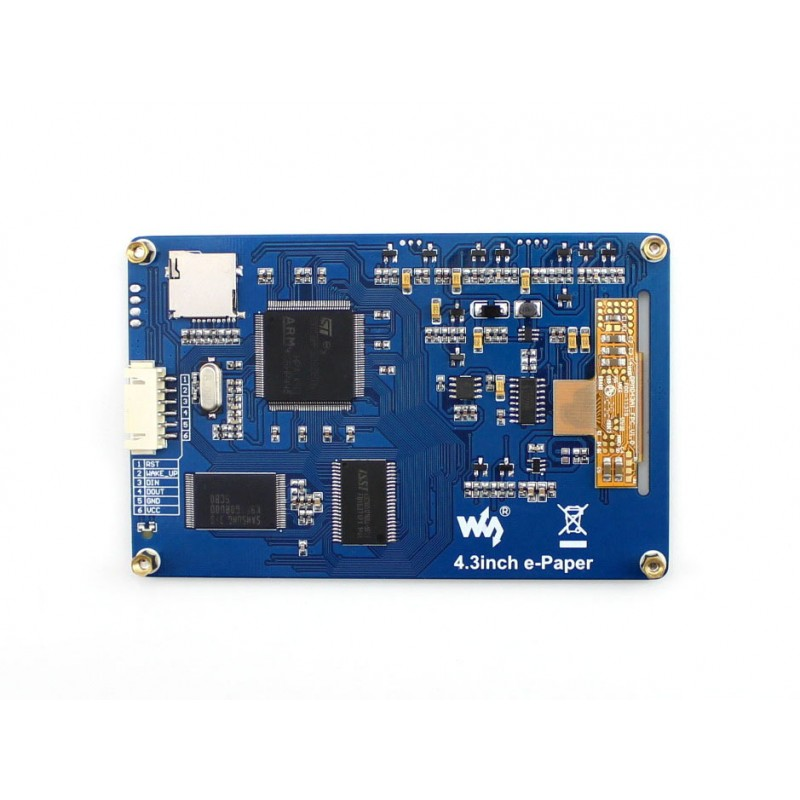
\includegraphics[scale=0.25]{43inch-e-paper-4back_waveshare_com}}
  }
  \caption{Waveshare e-Paper-Display}
  \label{pic:waveshare}
\end{figure}


\chapter{Aufbau und Grundlagen} %Vorläufiger Titel
Das \textsc{Beaglebone} wird mit \textsc{Ubuntu}-Linux und dem Kernel 4.1.12-ti-r29 betrieben. Allerdings ist der Treibercode nicht von einer speziellen Kernelversion, einer Linux-Distribution oder einem spezifischen Development-Board abhängig. 

Zuerst wurde für diese Arbeit zu Beginn ein \textsc{Arch}-Linux System mit einem Mainline-Kernel der Version 4.3 benutzt, da dieses Setup größtmögliche Freiheit in der Konfiguration des Systems und der Verwendung von \textsc{Custom-Kernels} bot. Leider gab es in dieser Konfiguration ein Problem bei der Verwendung der benötigten \texttt{UART}-Schnittstellen dessen Lösung den Rahmen dieser Arbeit sprengen würde und einen Wechsel unvermeidlich werden lies.

Der Treiber wird für die Kernelversionen 4.x der \textsc{ARM}-Plattform geschrieben und ist, solange es keine größeren Änderungen der verwendeten APIs gibt, für jeden entsprechenden Kernel kompilierbar.

\section{Aufbau der Hardware}
Das e-Paper Display besitzt ein \texttt{UART}-Interface %TODO Uart erklären
, welches die Kommunikation zwischen \textsc{Beaglebone} und Display über zwei Pins ermöglicht. Dazu wird die \texttt{DIN}-Leitung des Displays an den \texttt{TXD}-Pin des \texttt{UART-1}-Interface des \textsc{Beaglebones} angeschlossen. Ebenso wird mit der \texttt{DOUT}-Leitung und dem \texttt{RXD}-Pin des gleichen Interfaces verfahren. Die Leitungen \texttt{RST}, der Reset und \texttt{WAKEUP} des Displays werden an den \texttt{GPIO}\footnote{General Purpose Input/Output (Allzweck Ein-/Ausgabe), ein Pin dessen Verhalten frei programmiert werden kann}-Schnittstellen des \textsc{Beaglebone} angelegt und sorgen dafür, dass der Displayinhalt gelöscht, bzw. das Display aus einem Ruhezustand geholt werden kann. Zuletzt müssen noch Versorgungsspannung (\texttt{VCC}, 5V) und Erdung (\texttt{GND}) an die entsprechenden Pins des \textsc{Beaglebone} angeschlossen werden.  

Das \textsc{Beaglebone} selbst wird über ein USB-Kabel an den Hostrechner angeschlossen und kann darüber über das \texttt{ssh}-Protokoll erreicht werden. Um die zusätzliche Hardware versorgen zu können, muss das Board zusätzlich über ein 5V-Netzteil mit Strom versorgt werden. 

Um schon ab dem Bootvorgang Kernellogs zeitgleich lesen zu können wird die serielle Debugging-Schnittstelle des \textsc{Beaglebone} mithilfe eines USB-Serial-Wandlers und dem Programm \texttt{Minicom} ausgelesen. 

%TODO Bild Hardwareaufbau/Anschlüsse usw, 

%my screenshot
\begin{figure}[ht]
  \centering
  \fbox{
   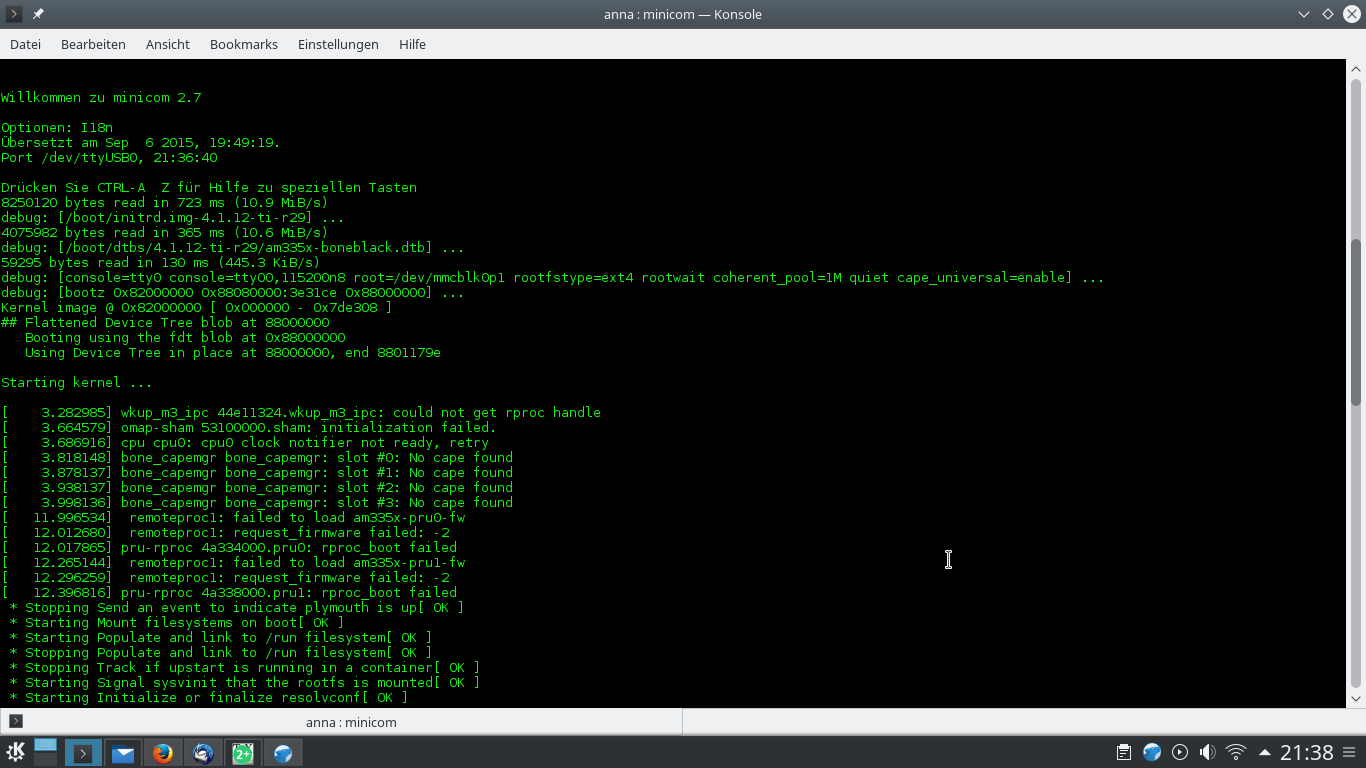
\includegraphics[scale=0.44]{minicom2}
  }
  \caption{Minicom Ausgabe während des Boot-Vorgangs}
  \label{pic:minicom}
\end{figure}

\section{Vorbereitungen zum Coding} %Titel ändern!
Kernelmodule müssen genau zu der Kernelversion, also den Schnittstellen des Kernels passen, auf dem sie ausgeführt werden sollen. Daher müssen die Quelltexte des Kernels vorliegen um dafür ein Kernelmodul zu erstellen. Sind Zielsystem des Treibers und dass auf dem das Modul kompiliert werden soll identisch, werden die Quelltexte traditionell unter \mintinline{bash}{/usr/src} abgelegt und mit dem \texttt{GCC}-Kompiler kompiliert.
Handelt es sich wie im Fall dieser Arbeit um unterschiedliche Plattformen und Kernelversionen, muss der Quelltext der genau passenden Kernelversion, sowie ein \texttt{GCC}-Compiler für die Zielplattform, ein \texttt{Cross-Compiler}, geladen werden. Natürlich kann auch direkt auf der Zielplattform, dem Beaglebone entwickelt werden, allerdings aufgrund dessen geringer Leistungsfähigkeit nicht empfehlenswert.

\subsection{Kernelquellen}
Für die hier verwendete Kernelversion können die Quelltexte wie folgende geladen und kompiliert werden. \texttt{CROSS\_COMPILE} gibt dabei an, welcher Cross-Compiler verwendet werden soll. Liegt dieser außerhalb der von \texttt{PATH}\footnote{Linux Umgebungsvariable, die alle Pfade enthält unter denen ausführbare Befehle gesucht werden} erfassten Pfade, muss hier der vollständige Pfad zum Cross-Compiler angegeben werden.

\begin{listing} [H]
\caption{Laden und Kompilieren der Kernelquellen}
\label{lst:getKernelsourcen}
\begin{minted} [frame=lines, framesep=2mm, fontsize=\footnotesize, linenos] {bash}
# Laden der Kernel-Quellen mit dem Versionsverwaltungssystem Git
git clone git@github.com:beagleboard/linux.git
cd linux
git checkout 4.1.12-ti-r29

# Laden der passenden Kernelkonfiguration für das Beaglebone
make ARCH=arm CROSS_COMPILE=arm-none-eabi- bb.org_defconfig
# Bau des Kernels und aller fest integrierter Module auf 4 Threads
make ARCH=arm CROSS_COMPILE=arm-none-eabi- -j4
# Bau der anderen Module (In-Tree)
make ARCH=arm CROSS_COMPILE=arm-none-eabi- modules -j4

# Soll der Kernel im Ganzen eingesetz werden, muss er mit folgenden Befehlen 
# auf die  SD-Karte des Beaglebone kopiert werden
make ARCH=arm CROSS_COMPILE=arm-none-eabi- INSTALL_MOD_PATH=/path/to/sdcard/usr modules_install
cp arch/arm/boot/zImage /path/to/sdcard/boot/
\end{minted}
\end{listing}

\subsection{Buildsystem}
Kernelmodule können entweder als fester Bestandteil des Kernels (In-Tree) oder als dynamisch ladbares Modul außerhalb des Kernels kompiliert werden. Im ersten Fall muss bei jeder Änderung der gesamte Kernel neu kompiliert und auf die SD-Karte des Beaglebone geladen werden, was aufgrund der Größe der Linux-Kernel-Quellen für Entwicklung und Testen eines neuen Treibers nicht zielführend ist. Treiber die in dieser Form in den Linux-Kernel eingebunden sind meist für Hardwarezugriffe verantwortlich die geschehen müssen, bevor der Kernel soweit hochgefahren ist um externe Module laden zu können. %Sicherheitsaspekte?
Für diese Projektarbeit soll mit der zweiten Möglichkeit, dem dynamisch ladbaren Modul, dass nur gegen die Kernelquellen gelinkt wird gearbeitet werden. Der Vorteil hierbei liegt zum einen darin, dass wirklich nur das Modul laufend neu kompiliert wird, zum anderen ist es so möglich im laufenden Betrieb das Modul zu entladen, gegen eine neuere Variante auszutauschen und wieder zum Kernel zu laden. 

Der Build des Linux-Kernels wird über das \texttt{GNU Make} Build-Management-System gesteuert, dass auch für das hier behandelte einzelne Kernel-Modul verwenden werden soll. Hierfür muss ein \texttt{Makefile} (M zwingend groß geschrieben) erstellt werden. Dass verwendete \texttt{Makefile} kann sowohl für ein In-Tree-Build, als auch wie in diesem Fall für ein konkretes Modul außerhalb der Kernelquellen verwendet werden. Um das Modul mit der richtigen Kernelversion zu verknüpfen, wird im Makefile der Pfad zu den Quelltexten angegeben. Stimmt die Kernelversion nicht genau überein, kann das Modul nicht geladen werden! 

Mit dem Aufruf von Make wird eine Objektdatei (\texttt{waveshare.o}) erzeugt die zusammen mit der Information über die Kernel-Version (\texttt{init/vermagic.o}) zum ladbaren Kernelmodul \texttt{waveshare.ko} gelinkt wird. %TODO Treiberbuch S 85 mitte 
\begin{listing} [H]
\caption{Makefile}
\label{lst:Makefile}
\begin{minted} [frame=lines, framesep=2mm, fontsize=\footnotesize, linenos] {make}
# Pfad zu den Kernelquellen
KERNEL_DIR=~/Development/linux

# Objektdatei
obj-$(CONFIG_WAVESHARE) += waveshare.o
obj-m := waveshare.o

# Speichert den Pfad von wo aus make aufgerufen wurde in PWD 
PWD := $(shell pwd)

# Ziel für make (all)
all:
	$(MAKE) -C $(KERNEL_DIR) SUBDIRS=$(PWD)

# Ziel für make modules
modules:
	$(MAKE) -C $(KERNEL_DIR) M=$(PWD) modules

# Ziel für make clean
clean: 
	$(MAKE) -C $(KERNEL_DIR) SUBDIRS=$(PWD) clean
	
\end{minted}
\end{listing}

%$ 

Das kompilierte Modul kann an jedem Ort liegen und mit \texttt{Root}-Rechten über den Befehl \mintinline{bash}{insmod waveshare.ko} (Pfadangabe ist erforderlich, falls das Modul nicht im aktuellen Verzeichnis liegt) zum Kernel geladen werden. Sollen auch eventuelle Abhängigkeiten des Moduls beim Laden beachtet werden oder das Modul Hotplugging unterstützen, muss das Modul im Zielsystem unter \mintinline{bash}{lib/modules/4.1.12-ti-r29/kernel/drivers/treibergattung} abgelegt und mit dem Befehl \mintinline{bash}{depmod -a} Abhängigkeiten aufgelöst sowie Map-Dateien für die Hotplugging-Infrastruktur erzeugt werden. %TODO depmod http://linux.die.net/man/8/depmod
Danach kann das Modul mit \texttt{Root}-Rechten und dem Befehl \mintinline{bash}{modprobe waveshare} geladen werden. Ist das Modul geladen, erscheint es in der Ausgabe von \mintinline{bash}{lsmod}. %TODO Ausgabe lsmod einfügen

%weiter in neuem Kapitel.. bin noch nicht glücklich mit dem ganzen in dieser aufteilung... evt auseinander ziehen, von einleitung weg





\newpage \appendix
%appendix
\addcontentsline{toc} {chapter} {Bibliografie}
%\bibliography{}
\listoflistings %auf deutsch umbenennen
\listoffigures %auf deutsch umbenennen
\end{document}